% Options for format can be included here
\documentclass{tikzposter}
\geometry{paperwidth=841mm,paperheight=1205mm}

\usepackage[english]{babel}

% Removing the watermark: still yet to decide if I really want to remove it
%	\tikzposterlatexaffectionproofoff

% Title, Author, Institute
\title{Data driven diagnosis of complex systems}
\author{Riccardo Orizio, Prof. Gregory Provan}
\institute{University College Cork}
\titlegraphic
{
	
\includegraphics[width=0.13\textwidth]{./Images/logo_sfi.png}
	\hspace{0.2\textwidth}
	
\includegraphics[width=0.13\textwidth]{./Images/logo_ucc.png}
	\hspace{0.2\textwidth}
	
\includegraphics[width=0.13\textwidth]{./Images/logo_lero.png}
}

% Title settings
% Rescaled all text by one factor in comparison to the original settings
\settitle
{
	\centering
	\vbox
	{
		\@titlegraphic \\[\TP@titlegraphictotitledistance]
		\centering
		\color{titlefgcolor}
		{\bfseries \huge \sc \@title \par}
		\vspace*{1em}
		{\LARGE \@author \par}
		\vspace*{1em}
		{\Large \@institute}
	}
}

% Choose Layout
%	\usetheme{Default}
%	\usetheme{Rays}			%	<--
%	\usetheme{Basic}
%	\usetheme{Simple}
\usetheme{Envelope}		%	<--
%	\usetheme{Wave}
%	\usetheme{Board}		%	<--
%	\usetheme{Autumn}
%	\usetheme{Desert}

%	\usecolorpalette
%	\usecolorpalette{Default}
%	\usecolorpalette{BlueGrayOrange}
%	\usecolorpalette{GreenGrayViolet}
%	\usecolorpalette{DPurpleGrayBlue}
%	\usecolorpalette{DBrownBlueOrange}

%	\usecolorstyle
%	\usecolorstyle{Default}
%	\usecolorstyle{Australia}	% <--
\usecolorstyle{Britain}		% <--
%	\usecolorstyle{Sweden}
%	\usecolorstyle{Spain}
%	\usecolorstyle{Russia}
%	\usecolorstyle{Denmark}
%	\usecolorstyle{Germany}

\begin{document}
	% Title block redimensioned due to length of the title
	\maketitle[width=0.9\textwidth]

	% General problem introduction
	\block{General Problem}
	{
		Performing diagnosis on a complex system requires at least an efficient
		and accurate model of the system itself, which can then be used to
		run simulations useful to collect data for diagnosis.
		The problem is that running simulations on such high fidelity models
		requires time and high performance resources, which cannot always be
		available.
		For this reason we want to generate a simple model of the complex system
		based only on real data, provided by the system itself, and then use it
		to perform our analysis.
		From such simple models we will be able to retrieve all information of
		the system requried to perform fault diagnosis on it.
		The data driven approach has attracted attention in the last years
		proving that it is an efficient tool to use in these scenarios, but
		other methods are still used, such as hierarchical models and reduced
		models.

		\begin{center}
			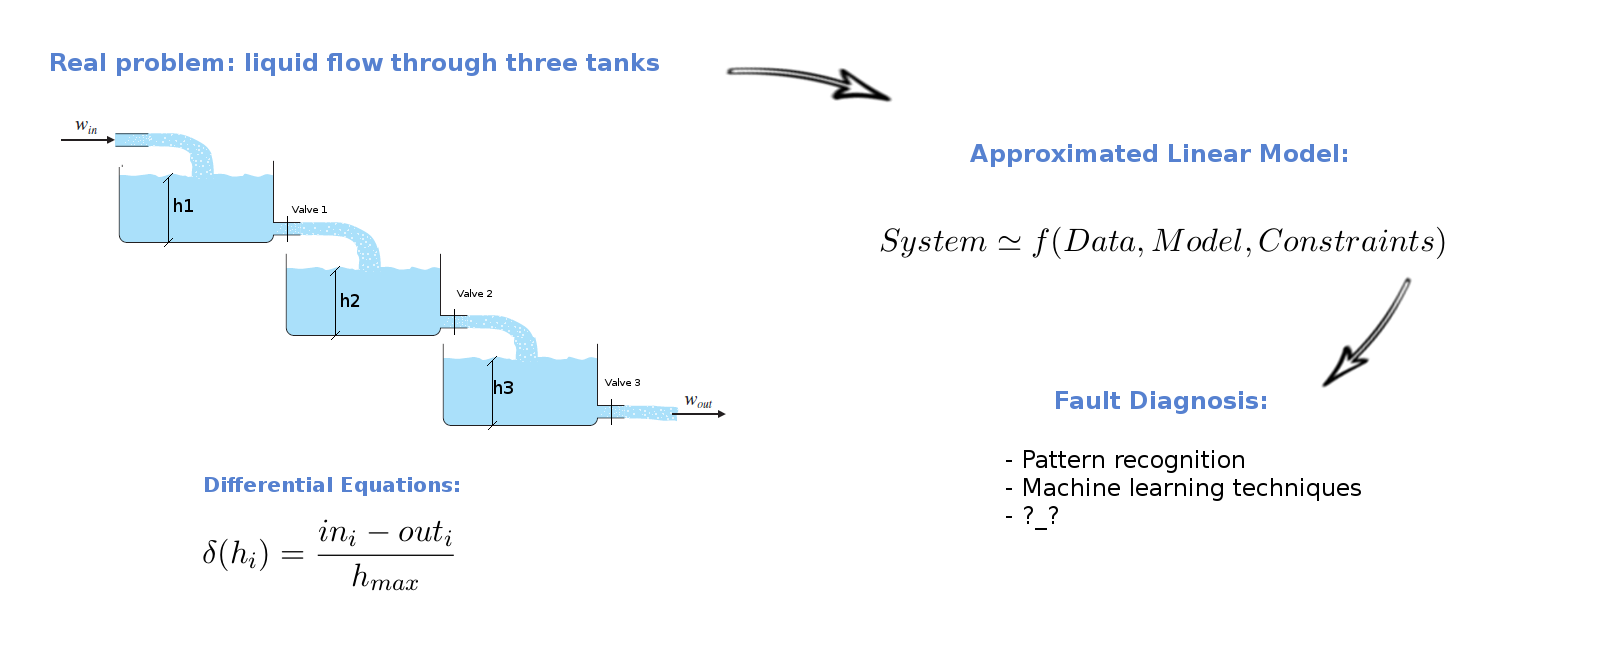
\includegraphics[width=0.75\textwidth]{./Images/3tanks.png}
		\end{center}
	}

	% Approach block
	\block{Approach}
	{
		Our goal is to create a framework able to create a diagnoser of the
		system under observation, only providing the data of its behaviour,
		either correct or faulty. \\
		
		% Cute paging of the steps to follow
		\begin{minipage}[t]{0.43\textwidth}
			\begin{center}
				\textbf{\textit{Model generation}}
			\end{center}
			The data driven model creation can be done using different
			approaches, from polynomial approaches to machine learning methods.
			The selection of the appropriate model to use will be done through
			an optimization problem based on \emph{Accuracy} and
			\emph{Computational Costs} of each model.
			$$ J(\cdot) = \alpha\ Accuracy(\cdot) + \beta\ Computational\ Cost(\cdot) $$
		\end{minipage}
		%%
		\hspace{15mm}
		%%
		\begin{minipage}[t]{0.43\textwidth}
			\begin{center}
				\textbf{\textit{Diagnosis}}
			\end{center}
			In respect to the error classification and recognition, a Neural
			Network or a series of Support Vector Machines will be implemeted to
			deal with the errors in the system behaviour.
		\end{minipage}
	}

	% Achievements block
	\block{Achievements}
	{
		Currently we are able to generate a linear model from the data of a
		high-fidelity model.
		Such models, or \emph{Corrective models}, properly approximate the
		behaviour of the high-fidelity models in each scenario separatedly, will
		that either be a normal or faulty behaviour.  
		The purpose of these corrective models have been extended to a more
		general scenario and try to generate the best models which can predict
		how to behave in each possible faulty situation.

		\begin{center}
			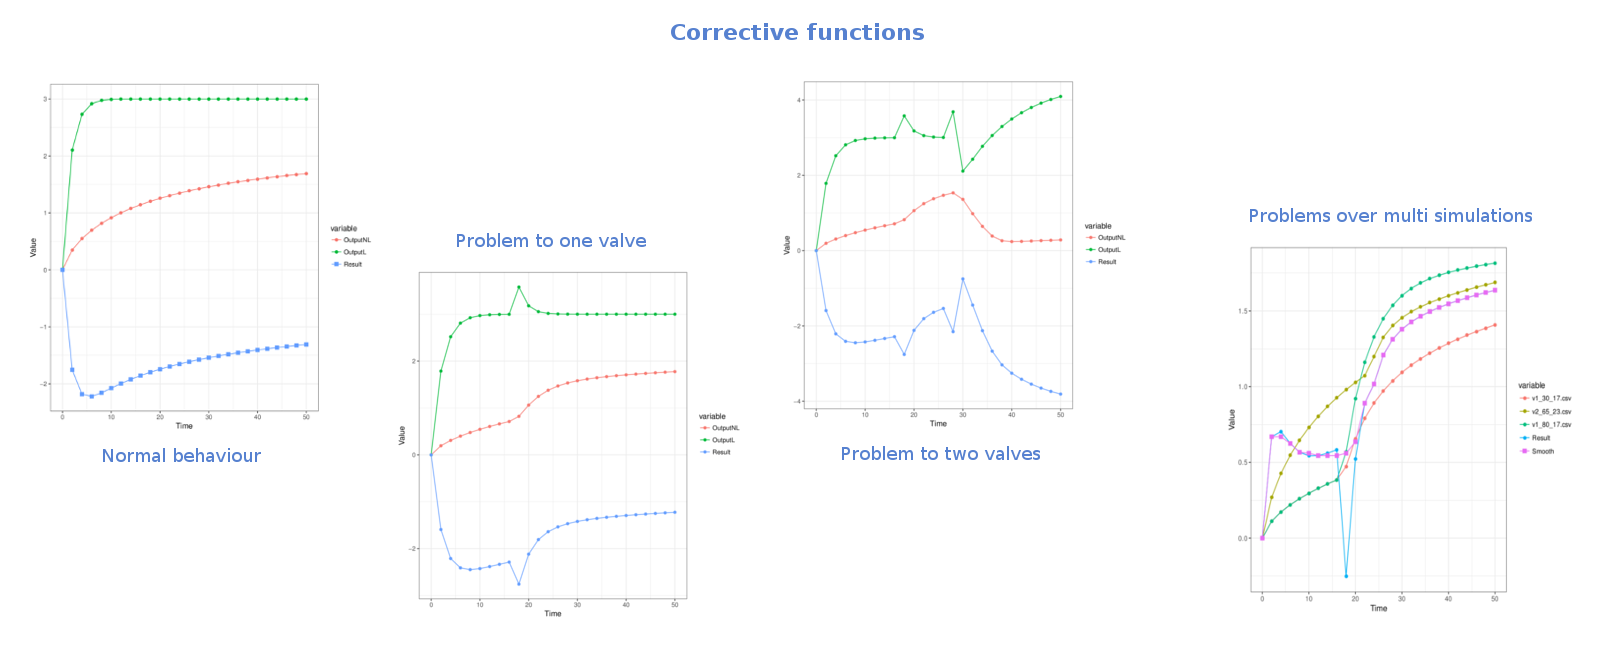
\includegraphics[width=0.75\textwidth]{./Images/Corrective_functions.png}
		\end{center}
	}

	% Next steps block
	\block{Next steps}
	{
		We are now trying to incorporate some basic machine learning concepts to
		our framework for the model generation, which will lead us to find which
		model is best to be used for a particular problem.
	}

\end{document}

